\section{Object Detectors}
This section will perform a technical analysis of the current primary \gls{cnn}-based object detectors.



\begin{comment}
	different approach to earlier two step methods
	inspired by recent SOTA classification networks that are fully convolutional
		resnets
	old approach to place a roi pooling layer between conv layers
		unnatural placement - speed cost
	r f-cn
		shared fc architecture
\end{comment}

\subsection{Regional Fully-Connected Network}
One of the current leading object detection methods is the \gls{rfcn} \cite{rfcn}, which as mentioned in \sectionref{related}, takes a different approach to that of the region-based methods such as Faster R-CNN. The authors of \gls{rfcn} were inspired by the recent advances in \gls{fcn} classification networks, such as ResNets, and argue that the addition of the \gls{roi}-pooling layer in the Faster R-CNN pipeline is unnatural and adds computational complexity. The authors hypothesise that the reasoning behind this addition is due to the trade-off between using a classification approach in an object detection pipeline. A defining factor in object detection is that the method should be able to respect translation variance, that translation of an object inside an object proposal should given a good indication as to how well the proposal fits the object. Whereas classification is more translation invariant, as the shifting of an object in an image does not effect how the system returns it's output. The use of the \gls{roi}-pooling layer placed in between convolutional layers means that any convolutions after this point are not translation invariant as it is not region specific. Rather than using this popular feature extractor, \gls{rfcn} uses position-sensitive score maps computed by a bank of convolutional layers. The maps add translation variance into the detection pipeline by computing scores in relation to position information with respect to the relative spatial position of an object. A \gls{roi}-pooling layer is added after the score-maps, however, no convolutional operations are done after this point ensuring translation variance.
\\\\
The overall approach of the \gls{rfcn} also consists of the popular two-stages of region proposal and region classification. Region proposal is done using the \gls{rpn} from Faster R-CNN followed by the position-sensitive score maps and \gls{roi} pooling for region classification. The overall architecture of the \gls{rfcn} can be seen in \figref{rfcnarch}.


\begin{figure}
  \caption{Architecture of \gls{rfcn}. Region proposals are found using the \gls{rpn} followed by classification based on a bank of position-sensitive score maps.}
  \centering
    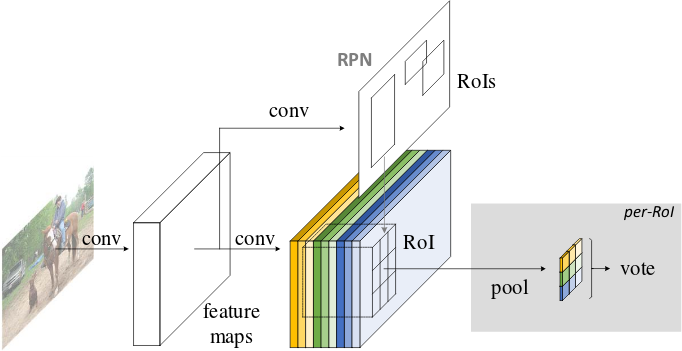
\includegraphics[width=0.8\textwidth]{Figs/Techanal/rfcnarchi.png}
    \label{fig:rfcnarch}
\end{figure}

The added translation variance post finding proposals with the \gls{rpn} is done by producing a bank of $k^2$ score maps for each object category. Therefore, there are a total of $k^2(C + 1)$ maps, where $C$ is the number of object categories plus one for a background class. The number of $k^2$ maps is due to a $k \times k$ spatial grid representing relative positions. Typically $k = 3$, therefore, the nine score maps represent position-sensitive scores for a given object category.